\originalchapter{8.421四份期中试卷}
以下题面按实际公开卷重编, 全部解答为编者补写. 没有在站点找到独立官方考试解答, 不把本章标作官方答案. 8.422大纲明确不设测验与期末, 因而不另造考试.
\originalsection{2008年期中}
\source{Midterm 2008, 第1题, V. Vuletić、W. Ketterle.}
\begin{exercise}正电子素由电子和正电子组成. (a) $s$态低场与任意$l$高场量子数; (b) $1s$各超精细态在极低、极高场的磁矩, 以Bohr磁子表示; (c) 画能级对$B$, 标简并与两端量子数; (d) 高场Zeeman及超精细能, 可留一个超精细系数; (e) 有限场是否简并, 原因是什么?\end{exercise}
\begin{solution}忽略湮灭宽度、异常磁矩与轨道抗磁修正, $H=A\mathbf s_e\cdot\mathbf s_p/\hbar^2+2\mu_BB(s_{ez}-s_{pz})/\hbar$. (a) 低场$s$态为$F=0,1,m_F$; 高场为$n,l,m_l,m_{se},m_{sp}$, 等质量反号电荷使一阶轨道Zeeman相消. (b,c) $m_F=\pm1$始终$E=A/4$, 斜率0; $m_F=0$两支$E=-A/4\pm\sqrt{A^2/4+4\mu_B^2B^2}$. 低场四态斜率全0, 高场两$m=0$支斜率$\pm2\mu_B$, 连接$\ket{\uparrow_e\downarrow_p}$与$\ket{\downarrow_e\uparrow_p}$; 两平行自旋态斜率0. 这些解析曲线给完整图形, 上支自$F=1,m=0$弯上, 下支自$F=0$弯下, $m=\pm1$水平. (d) $E_Z=2\mu_BB(m_{se}-m_{sp})$, $E_{
m hf}=Am_{se}m_{sp}$, 若$l>0$还须允许其他细结构耦合, 本式是题问自旋超精细领先项. (e) $m_F=\pm1$在有限场仍简并, 因两相反磁矩的平行自旋贡献相消; 其他两支在$B\ne0$不与其相交.
\end{solution}
\source{Midterm 2008, 第2题.}
\begin{exercise}氢先按无自旋点电子、点核非相对论模型. (a) 量子数范围及简并; (b) 电子有小有限体积怎样移能; (c) 只有核有自旋磁矩、电子无自旋时Hamiltonian与好量子数; (d) 只有电子有自旋磁矩时怎样改变, 相对论描述又如何?\end{exercise}
\begin{solution}(a) $n\ge1,l=0,\ldots,n-1,m=-l,\ldots,l$, 能量仅依$n$, 简并$n^2$. (b) 若有限体积表示球对称电荷分布, 短程库仑吸引被平滑, 主要$S$态向上接触位移, 消去同$n$不同$l$简并但不劈裂$m$. 未给形状不能定量. (c) 核磁矩与电子轨道磁场耦合$\mathbf I\cdot\mathbf L$及可能核四极, 好量子数$\mathbf F=\mathbf L+\mathbf I$与$m_F$; $l=0$没有由无自旋电子产生的磁接触作用. (d) 自旋轨道作用使$j=l\pm1/2$分裂, 自旋不耦合时只是倍增简并. 相对论还带动能与Darwin项, 合并后Dirac能量依$n,j$, 不能单独只加自旋轨道而称完整相对论谱.
\end{solution}
\source{Midterm 2008, 第3题.}
\begin{exercise}等权二态在$d=1,2,3$维热腔, 激发能$\hbar\omega$. (a) 热布居比; (b) 各维辐射谱能量密度; (c) Einstein系数关系. 低维可由压缩三维腔的方向实现.\end{exercise}
\begin{solution}(a) $N_e/N_g=\e^{-\hbar\omega/k_BT}$. (b) 保留$p_d$个实际传播偏振时, 每$d$维体积每角频率模密度为
\[D_d=\frac{p_dS_{d-1}\omega^{d-1}}{(2\pi)^dc^d},\qquad S_0=2,\ S_1=2\pi,\ S_2=4\pi.\]
 能量密度$u_d=\hbar\omega D_d/(\e^{\hbar\omega/k_BT}-1)$. 所以$d=1$为$p_1\hbar\omega/(\pi c)$乘Bose因子; $d=2$为$p_2\hbar\omega^2/(2\pi c^2)$; $d=3,p_3=2$为$\hbar\omega^3/(\pi^2c^3)$. 真实薄腔的截止、偏振和单位体积换算须指定, 不能无条件套$d-1$偏振使一维无光. (c) 详细平衡给$B_{ge}=B_{eg}$,$A/B=\hbar\omega D_d$. 简并不等时补$g_gB_{ge}=g_eB_{eg}$.
\end{solution}
\source{Midterm 2008, 第4题.}
\begin{exercise}$S<P<D$, 跃迁$\omega_{SP},\omega_{PD}$, 偶极$d_{SP},d_{PD}$. (a,b) 不作旋波写$S,P$光移; (c) $\omega_{SP}=2\omega_{PD},d_{SP}=2d_{PD}$时求magic光频.\end{exercise}
\begin{solution}作业五第2题的完整反旋式给$U_S=-Kd_{SP}^2F(\omega_{SP})$,$U_P=K[d_{SP}^2F(\omega_{SP})-d_{PD}^2F(\omega_{PD})]$. 取$f=2,n=2$, 得$\omega^2/\omega_{PD}^2=4/5$, 即$\omega=2\omega_{PD}/\sqrt5$. 偶极大小和光强抵消, 只决定共同阱深.
\end{solution}
\source{Midterm 2008, 第5题.}
\begin{exercise}自旋$1/2$初态为$z$本征态, 可加静态或时变$z$和横向磁场. 描述三种概念不同的方式把一半布居转至另一$z$态, 明确时间依赖.\end{exercise}
\begin{solution}一是保持$B_z$、施共振横向旋转场$B_1(\cos\omega_0t,\sin\omega_0t)$, 开$\pi/(2\Omega)$时长即$\pi/2$脉冲. 二是突然关闭$B_z$、打开静态$B_x$, 绕$x$转$\pi/2$后关横场并恢复$B_z$. 三是从沿$z$的有限场开始, 缓慢把方向旋至横向并保持总场不为零, 使态绝热跟随, 再突然恢复$z$测量轴, 横向纯态对$z$两结果各半. 三者分别利用共振驱动、自由进动和绝热轴跟随, 不能只换脉冲长度算三方法.
\end{solution}

\originalsection{2010年期中}
\source{Midterm 2010, 第1题.}
\begin{exercise}(a) 给$^2S_{1/2},^3S_1,^1D_2,^3P_0$磁矩或$g$; (b) 两负电粒子自旋$s_1,s_2$,$\boldsymbol\mu_i=-g_i\mu_B\mathbf s_i/\hbar$, 耦合总$J$. 弱$z$场求能级与合成$g_J$, 分别$g_1=g_2$, $g_1=-g_2$, $g_2=0$.\end{exercise}
\begin{solution}(a) $g$依次2,2,1; $J=0$态无一阶磁矩, $g$商式不定义. 磁矩向量$-g\mu_B\mathbf J/\hbar$. (b) 设$C=J(J+1)$,$C_i=s_i(s_i+1)$, 投影$\mathbf s_i$到$J$给$g_J=[g_1(C+C_1-C_2)+g_2(C-C_1+C_2)]/(2C)$, 能量$E_{Jm}=E_J+g_J\mu_BmB$. 三情形分别为$g_1$, $g_1(C_1-C_2)/C$, $g_1(C+C_1-C_2)/(2C)$. $J=0$一阶移位零; 弱场还要求未被磁场显著混合不同$J$多重态.
\end{solution}
\source{Midterm 2010, 第2题.}
\begin{exercise}(a) 弱单色共振驱动$\omega_R$, 自然宽$\Gamma$, 激发率量级; (b) 它怎样依赖偶极矩阵元, 宽带是否同样; (c) 无限强度激发散射率与截面; (d) 非相对论氢样波函数中$2p_{1/2}\to1s_{1/2}$,$2s_{1/2}\to1s_{1/2}$,$3d_{3/2}\to2s_{1/2}$,$2p_{3/2}\to2p_{1/2}$,$3d_{3/2}\to2p_{1/2}$的主多极.\end{exercise}
\begin{solution}(a) $R\sim\omega_R^2/\Gamma$. (b) $\omega_R^2\propto d^2I$, $\Gamma\propto d^2\omega_0^3$, 同频不同偶极的单色共振弱场截面领先项不依$d$. 宽带$R\sim\omega_R^2/\Gamma_L$, 宽度由光决定, 因而正比$d^2$. (c) 净吸收后的稳态散射最多$\Gamma/2$, 截面随$I^{-1}\to0$; 单独“总吸收跃迁数”在强场包含大量受激来回, 与净散射不同. (d) 依次E1; $2s\to1s$单光子E1禁戒且M1径向正交, 主为两E1光子的二阶过程; E2; M1角动量允许; E1. 若严格不含精细结构, 两$2p_j$同能, 第四条实际无有限频率辐射, “M1”只给其角选择规则, 非零频率须结构劈裂.
\end{solution}
\source{Midterm 2010, 第3题.}
\begin{exercise}锂核$Z=3$和负muon,$m_\mu/m_e=207$, 忽略核质量修正. (a) 推$a_0$; (b) 轨道半径和$1s$束缚能相对氢; (c) 同$Z$电子、muon相对论束缚修正之比; (d) 三电子锂与换一个muon的基态能, 单位Ry, 忽略粒子间相互作用; (e) 至少三种主要只影响$S$的机制.\end{exercise}
\begin{solution}(a) 动能$\hbar^2/(mr^2)$与$Ze^2/(4\pi\epsilon_0r)$平衡得$r\sim a_0/Z$. (b) muon半径$a_0/(3\times207)$, 结合能$9\times207$ Ry. (c) 绝对相对论修正正比质量, 比207; 相对于各自束缚能的比例均$(Z\alpha)^2$, 比1. (d) 电子两占$1s$一占$n=2$, 能$-9(2+1/4)=-20.25$ Ry. 换muon可让它占独立$1s$, 两电子均$1s$, 能$-9(207+2)=-1881$ Ry. (e) Darwin接触项、有限核大小领先项、接触超精细作用. Lamb位移对$S$尤其大但也影响非$S$, 不能把它严格说成“仅$S$”.
\end{solution}

\originalsection{2012年期中}
\source{Midterm 2012, 第1题.}
\begin{exercise}电子轨道$L$, 自旋$S$, 核$I$. (a) 极强磁场的量子数与能量; (b) 横向振荡场连哪些态; (c) $L=0,H_{\rm hf}=A\mathbf S\cdot\mathbf I/\hbar^2$, 一阶能量; (d,e) $S=I=1/2,A>0$画随场能级、标态与横场矩阵元; (f) 任意$S,I$的一阶混合波函数; (g) 用混合讨论$1/2,1/2$的新跃迁及矩阵元.\end{exercise}
\begin{solution}(a) 好量子数$m_L,m_S,m_I$, $E_Z=\mu_BB(g_Lm_L+g_Sm_S+g_Im_I)$, 加小的结构修正. (b) 横场每次改变其中一个投影$\pm1$, 矩阵元$g_j\mu_BB_\perp\sqrt{j(j+1)-m_j(m_j\pm1)}/2$. (c) 超精细一阶对角$Am_Sm_I$. (d) 对$L=0$,$I=S=1/2$, 伸展两态$E=A/4\pm\mu_BB(g_S+g_I)/2$,$m=0$两态$E=-A/4\pm\sqrt{A^2+[(g_S-g_I)\mu_BB]^2}/2$. 低场分别$F=1$三态与$F=0$, 高场恢复两个投影. 横场$\Delta m=\pm1$, 即伸展态连两$m=0$混合态; 两伸展态彼此$\Delta m=2$不直接连. (e) 可给四条线的精确矩阵元. 令$\delta=(g_S-g_I)\mu_BB>0$, $\tan2\theta=A/\delta$, $0<\theta\le\pi/4$, 两$m=0$态为$u=\cos\theta\,\uparrow\downarrow+\sin\theta\,\downarrow\uparrow$, $v=-\sin\theta\,\uparrow\downarrow+\cos\theta\,\downarrow\uparrow$. 对横场$H_\perp=\mu_BB_\perp(g_SS_x+g_II_x)/\hbar$, 以$\mu_BB_\perp/2$为公因子, 得
\[\begin{array}{c|cc}
 &u&v\\\hline
 \uparrow\uparrow&g_I\cos\theta+g_S\sin\theta&g_S\cos\theta-g_I\sin\theta\\
 \downarrow\downarrow&g_S\cos\theta+g_I\sin\theta&g_I\cos\theta-g_S\sin\theta
\end{array}\]
高场$\sin\theta\simeq A/(2\delta)$, 主电子翻转和核翻转分别趋$g_S\mu_BB_\perp/2$与$g_I\mu_BB_\perp/2$.

(f) 非简并高场微扰为$\ket{m_S,m_I}+\sum_{\pm}c_\pm\ket{m_S\pm1,m_I\mp1}$, 其中
\[c_\pm=\frac{(A/2)\sqrt{S(S+1)-m_S(m_S\pm1)}\sqrt{I(I+1)-m_I(m_I\mp1)}}{\mp(g_S-g_I)\mu_BB}.\]
同$m_S+m_I$才混合. (g) $1/2$情形混合量级$A/[(g_S-g_I)\mu_BB]$. 原来纯核翻转的弱线可借电子矩阵元获得附加振幅约$g_S\mu_BB_\perp A/[4(g_S-g_I)\mu_BB]$, 与直接核项相干相加; 其符号依两$m=0$支. 所有四条伸展态到$m=0$线均可出现, 但$\Delta m$为0或2的新横场线仍不允许. 下图实际绘出(d)四支, 不以混合消除总投影选择规则.
\end{solution}

\begin{center}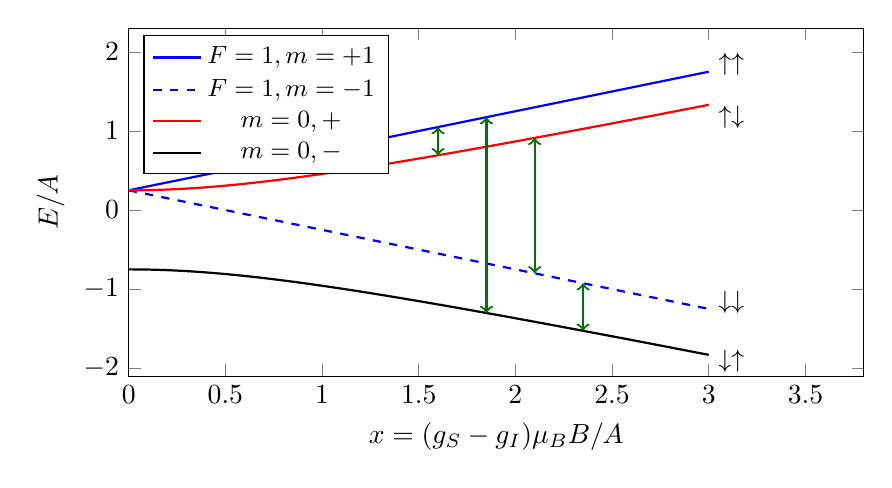
\begin{tikzpicture}
\begin{axis}[width=.9\linewidth,height=6cm,xlabel={$x=(g_S-g_I)\mu_BB/A$},
 ylabel={$E/A$},xmin=0,xmax=3.8,ymin=-2.1,ymax=2.3,
 domain=0:3,samples=81,legend style={font=\small,at={(.02,.98)},anchor=north west}]
\addplot[blue,thick]{.25+x/2};\addlegendentry{$F=1,m=+1$}
\addplot[blue,dashed,thick]{.25-x/2};\addlegendentry{$F=1,m=-1$}
\addplot[red,thick]{-.25+sqrt(1+x^2)/2};\addlegendentry{$m=0,+$}
\addplot[black,thick]{-.25-sqrt(1+x^2)/2};\addlegendentry{$m=0,-$}
\node[right,font=\small] at(axis cs:3,1.85){$\uparrow\uparrow$};
\node[right,font=\small] at(axis cs:3,1.18){$\uparrow\downarrow$};
\node[right,font=\small] at(axis cs:3,-1.16){$\downarrow\downarrow$};
\node[right,font=\small] at(axis cs:3,-1.91){$\downarrow\uparrow$};
\draw[<->,thick,green!45!black](axis cs:1.6,1.05)--(axis cs:1.6,.6934);
\draw[<->,thick,green!45!black](axis cs:1.85,1.175)--(axis cs:1.85,-1.3015);
\draw[<->,thick,green!45!black](axis cs:2.1,-.8)--(axis cs:2.1,.9130);
\draw[<->,thick,green!45!black](axis cs:2.35,-.925)--(axis cs:2.35,-1.5265);
\end{axis}\end{tikzpicture}\end{center}
图为忽略微小$g_I/g_S$斜率修正的示意解析曲线, 用上文全式可恢复核Zeeman项. 低场$m=0,+$为$(\uparrow\downarrow+\downarrow\uparrow)/\sqrt2$的$F=1$态, $m=0,-$为反对称$F=0$态; 右端箭头标明高正场的电子/核投影. 绿色四箭头均为横场$\Delta m=\pm1$跃迁, 没有伸展态间$\Delta m=2$线.

\source{Midterm 2012, 第2题.}
\begin{exercise}(a) 无耦合原子单模腔联合基态; (b) 有限电偶极耦合的领先基态与能量; (c) 自由空间是否类似; (d) 初态$e\otimes(a_1\ket1+a_2\ket2)$, 腔远失谐, 忽略上态耗尽且用RWA, 求随时间联合态.\end{exercise}
\begin{solution}(a) $\ket{g,0}$. (b) 若仅JC旋波Hamiltonian, 这个态仍精确基态且无修正; 原题本问有限全偶极作用需含反旋项$\hbar g a^\dagger\sigma_+$. 二阶得$\ket G\simeq\ket{g,0}-g\ket{e,1}/(\omega_c+\omega_0)$, $\Delta E=-\hbar g^2/(\omega_c+\omega_0)$, 归一化修正为二阶. 完整规范模型还需相应自能或$A^2$项, 不能凭单模截断计算绝对可观测Lamb位移. (c) 自由空间虚光子模也带来辐射能移, 需重整化处理. (d) 取$\delta=\omega_c-\omega_0$, 上态每$n$光子的位移$-\hbar g^2(n+1)/\delta$. 故$\psi\simeq\sum_{n=1,2}a_n\exp\{-\ii[n\omega_c+\omega_0/2-g^2(n+1)/\delta]t\}\ket{e,n}$, 忽略$O(g\sqrt{n+1}/\delta)$的$g,n+1$幅度. 场叠加的相对相位被原子色散作用改变.
\end{solution}
\source{Midterm 2012, 第3题.}
\begin{exercise}(a) 远失谐光在基态混10\%激发布居, 激发寿命$\tau$, 用RWA求散射率; (b) 极大驱动时最低缀饰态及散射率.\end{exercise}
\begin{solution}(a) 共振邻域的RWA与Markov模型给$0.1/\tau$; 若频率远至反旋不可忽略, 还需频率依赖辐射率, 与题设RWA冲突不可偷偷延伸. (b) 共振且驱动主导时最低支约$(\ket g-\e^{\ii\phi}\ket e)/\sqrt2$, 散射率$1/(2\tau)$.
\end{solution}
\source{Midterm 2012, 第4题.}
\begin{exercise}新的正电粒子自旋$1/2$, 满投影磁矩$+2\mu_B$, 与普通电子形成类氢原子. 求$1s$超精细态低、高场磁矩.\end{exercise}
\begin{solution}电子满投影磁矩$-\mu_B$, 新粒子为$+2\mu_B$. 低场$F=1,m=\pm1$的实际磁矩为$\pm\mu_B$, $m=0$与单态为0, 能量斜率与磁矩相反. 高场四直积的实际磁矩为$+\mu_B,-\mu_B,+3\mu_B,-3\mu_B$, 分别对应两平行与两反平行自旋. 若题采用$\partial E/\partial B$称磁矩, 全部符号反转; 本卷明确使用$\mu=-\partial E/\partial B$的物理磁矩约定.
\end{solution}
\source{Midterm 2012, 第5题.}
\begin{exercise}氢基态电子特征速度, 高核电荷$Z$与大$n$Rydberg速度, 换约200倍重的muon怎样变化?\end{exercise}
\begin{solution}$v\sim\alpha c$,$v_n\sim Z\alpha c/n$. 同$Z,n$时质量约去, muon轨道缩小、束缚能增加而速度不变. 要求$Z\alpha\ll1$以使用非相对论尺度.
\end{solution}

\originalsection{2014年期中}
\source{Midterm 2014, 第1题.}
\begin{exercise}Dirac氢$n=2$哪两态简并? Lamb、Darwin、质子大小、质子质量、自旋轨道各是否解除, 为什么? $n=2$Lamb约1 GHz, 估$n=1$. 怎样实验区分Lamb与核大小?\end{exercise}
\begin{solution}$2S_{1/2},2P_{1/2}$简并. 辐射Lamb与有限核大小解除, 后者主要接触$S$; Darwin、自旋轨道已包含于Dirac低能展开, 单独看可能移位不同, 但连同相对论动能合并后保留该简并, 不可再重复加一次. 简单有限质量的约化质量替换不解除; 更高阶反冲可有小劈裂, 须区分版本. $S$原点密度按$n^{-3}$, 估$1S$约8 GHz, 辐射对数因子使之非精确8倍. 用不同$l$与不同$n$跃迁并结合独立核半径或同位素测量拟合不同依赖, 因Lamb也作用非$S$, 而核大小领先为$S$接触项; 单一$1S-2S$频率不能唯一分离两未知修正.
\end{solution}
\source{Midterm 2014, 第2题.}
\begin{exercise}$\mathbf J=\mathbf L+\mathbf S$, 电子$g_e=2$. (a) $S=0,L=0,L=S$的$g$; (b) 推一般$L,S,J$磁矩.\end{exercise}
\begin{solution}磁矩$-\mu_B(\mathbf L+2\mathbf S)/\hbar$. 用$\mathbf L\cdot\mathbf J=[J^2+L^2-S^2]/2$及另一投影, 得$g_J=1+[J(J+1)+S(S+1)-L(L+1)]/[2J(J+1)]$. 三种$J\ne0$情形为1,2,3/2. $J=0$态磁矩零, 不由商式定义$g$.
\end{solution}
\source{Midterm 2014, 第3题.}
\begin{exercise}(a) 无自旋$S$基态与$P$激发多重态, 先画零、高$B$态, 比较$E\parallel B$及$E\perp B$的耦合、Zeeman符号、领先Stark位移, 零、高場差别与高场须加何项; (b) 无自旋正电子素$P$的Zeeman与前例不同? (c) 大$n$Rydberg $S$极化率, 主要耦合同$n$的$P$, 随$n$尺度; (d) 线性Stark阈值尺度.\end{exercise}
\begin{solution}取$B\parallel z$, 零场三个$P,m=0,\pm1$简并; 电子磁矩负, 能移为$+m\mu_BB$. 设零场$P-S$间隔$\hbar\omega_0$, 单方向偶极$d$. 平行电场只连$m=0$, $U_\parallel=-d^2E^2/(\hbar\omega_0)$. 垂直场两圆分量各一半,$U_\perp=-d^2E^2[1/(\hbar\omega_0+\mu_BB)+1/(\hbar\omega_0-\mu_BB)]/2$. 零场相等, 有场因分母不同而各向异性, 靠近交叉需简并处理. 强磁场还须加$e^2B^2r_\perp^2/(8m)$的抗磁项, 若超过Coulomb尺度原$S,P$标签也会混合. 正电子素的等质量反号电荷使轨道线性Zeeman相消, 仍有二次抗磁作用.

Rydberg同$n$近邻异宇称能隙$\Delta E\sim n^{-3}$, 偶极$d\sim ea_0n^2$, 故$\alpha\sim d^2/\Delta E\sim n^7$. 线性强混合阈值$E_c\sim\Delta E/d\sim n^{-5}$. 严格氢的无修正同$n$简并会在任意弱场出现线性Stark, 必须有量子亏损、Lamb或其他劈裂才有本题$n^{-3}$有限阈值.
\end{solution}

\begin{center}\begin{tikzpicture}[>=Stealth,x=1cm,y=1cm]
\node at(1.4,3.0){零场};\node at(6.1,3.0){已分辨Zeeman劈裂};
\draw[thick](0,0)--(2.8,0) node[right]{$S,m=0$};
\draw[thick](0,2)--(2.8,2);
\node[above] at(1.4,2){$P,m=-1,0,1$};
\draw[->,blue,thick](.6,.08)--(.6,1.92);
\draw[->,red,dashed,thick](1.8,.08)--(1.8,1.92);
\node[blue] at(.55,1){$\parallel$};\node[red] at(2.2,1){$\perp$};
\draw[thick](4.4,0)--(7.5,0) node[right]{$S,0$};
\draw[thick](4.4,1.3)--(7.5,1.3) node[right]{$P,-1$};
\draw[thick](4.4,2)--(7.5,2) node[right]{$P,0$};
\draw[thick](4.4,2.7)--(7.5,2.7) node[right]{$P,+1$};
\draw[->,blue,thick](5.2,.08)--(5.2,1.92);
\draw[->,red,dashed,thick](6.3,.08)--(6.3,1.22);
\draw[->,red,dashed,thick](7.0,.08)--(7.0,2.62);
\node[blue] at(5.1,.7){$\pi$};
\node[red] at(6.5,1.8){$\sigma^\mp$};
\end{tikzpicture}\end{center}
蓝色为$E\parallel B$的$\Delta m=0$, 红色为$E\perp B$的$\Delta m=\pm1$两分量. 右图仍在轨道量子数可用、抗磁混合未占主导的区间; 极高场需上文的二次项, 不再由三条直线完整表示.

\source{Midterm 2014, 第4题.}
\begin{exercise}(a) 单模体积$V$, 偶极$d$, 频率$\omega$, 饱和所需光子数用特征速率比表达, 可略2因子; (b) 对$d,V,\omega$尺度; (c) 单光子能否饱和; (d) 黑体腔每共振模饱和占据与温度, 此处保留数因子; (e) 模密度与能激发原子的共振模数及尺度; (f) 比较单模和黑体.\end{exercise}
\begin{solution}(a) 单光子耦合$g=d\sqrt{\hbar\omega/(2\epsilon_0V)}/\hbar$, 经典$n$光子驱动$\Omega\sim2g\sqrt n$, $s\sim\Omega^2/\Gamma^2$, 所以$n_s\sim(\Gamma/g)^2$. (b) $\Gamma\propto d^2\omega^3$, $g^2\propto d^2\omega/V$, 得$n_s\propto d^2V\omega^5$. (c) 强耦合小体积腔可使$n_s\lesssim1$, 但单光子不可当固定经典连续驱动, 应用JC动力学判定交换和饱和响应. (d) 宽带Einstein模型$s=2\bar n$, 饱和每模$\bar n=1/2$, 因而$T_s=\hbar\omega/(k_B\ln3)$. (e) 每角频率模密度$V\omega^2/(\pi^2c^3)$, 原子有效宽$\Gamma$, 模数量级$M=V\omega^2\Gamma/(\pi^2c^3)\propto Vd^2\omega^5$. 有限离散腔须足够密才可用连续密度. (f) 黑体每模只需固定占据, 但有$M$个模一起作用; 总共振光子数约$M/2$与单模$n_s$同尺度. 单模集中驱动与宽带多数模的分配不同, 不表示黑体总资源独立于腔体积.
\end{solution}
